\ifx\wholebook\relax\else

% --------------------------------------------
% Lulu:

    \documentclass[a4paper,12pt,twoside]{../includes/ThesisStyle}

	\usepackage[T1]{fontenc} %%%key to get copy and paste for the code!
%\usepackage[utf8]{inputenc} %%% to support copy and paste with accents for frnehc stuff
\usepackage{times}
\usepackage{ifthen}
\usepackage{xspace}
\usepackage{alltt}
\usepackage{latexsym}
\usepackage{url}            
\usepackage{amssymb}
\usepackage{amsfonts}
\usepackage{amsmath}
\usepackage{stmaryrd}
\usepackage{enumerate}
\usepackage{cite}
%\usepackage[pdftex,colorlinks=true,pdfstartview=FitV,linkcolor=blue,citecolor=blue,urlcolor=blue]{hyperref}
\usepackage{xspace}
%\usepackage{graphicx}
\usepackage{subfigure}
\usepackage[scaled=0.85]{helvet}
        
        
\newcommand{\sepe}{\mbox{>>}}
\newcommand{\pack}[1]{\emph{#1}}
\newcommand{\ozo}{\textsc{oZone}\xspace}
\newcommand\currentissues{\par\smallskip\textbf{Current Issues -- }}

\newboolean{showcomments}
\setboolean{showcomments}{true}
\ifthenelse{\boolean{showcomments}}
  {\newcommand{\bnote}[2]{
	\fbox{\bfseries\sffamily\scriptsize#1}
    {\sf\small$\blacktriangleright$\textit{#2}$\blacktriangleleft$}
    % \marginpar{\fbox{\bfseries\sffamily#1}}
   }
   \newcommand{\cvsversion}{\emph{\scriptsize$-$Id: macros.tex,v 1.1.1.1 2007/02/28 13:43:36 bergel Exp $-$}}
  }
  {\newcommand{\bnote}[2]{}
   \newcommand{\cvsversion}{}
  } 


\newcommand{\here}{\bnote{***}{CONTINUE HERE}}
\newcommand{\nb}[1]{\bnote{NB}{#1}}
\newcommand{\fix}[1]{\bnote{FIX}{#1}}
%%%% add your own macros 

\newcommand{\sd}[1]{\bnote{Stef}{#1}}
\newcommand{\ja}[1]{\bnote{Jannik}{#1}}
\newcommand{\na}[1]{\bnote{Nico}{#1}}
%%% 


\newcommand{\figref}[1]{Figure~\ref{fig:#1}}
\newcommand{\figlabel}[1]{\label{fig:#1}}
\newcommand{\tabref}[1]{Table~\ref{tab:#1}}
\newcommand{\layout}[1]{#1}
\newcommand{\commented}[1]{}
\newcommand{\secref}[1]{Section \ref{sec:#1}}
\newcommand{\seclabel}[1]{\label{sec:#1}}

%\newcommand{\ct}[1]{\textsf{#1}}
\newcommand{\stCode}[1]{\textsf{#1}}
\newcommand{\stMethod}[1]{\textsf{#1}}
\newcommand{\sep}{\texttt{>>}\xspace}
\newcommand{\stAssoc}{\texttt{->}\xspace}

\newcommand{\stBar}{$\mid$}
\newcommand{\stSelector}{$\gg$}
\newcommand{\ret}{\^{}}
\newcommand{\msup}{$>$}
%\newcommand{\ret}{$\uparrow$\xspace}

\newcommand{\myparagraph}[1]{\noindent\textbf{#1.}}
\newcommand{\eg}{\emph{e.g.,}\xspace}
\newcommand{\ie}{\emph{i.e.,}\xspace}
\newcommand{\ct}[1]{{\textsf{#1}}\xspace}


\newenvironment{code}
    {\begin{alltt}\sffamily}
    {\end{alltt}\normalsize}

\newcommand{\defaultScale}{0.55}
\newcommand{\pic}[3]{
   \begin{figure}[h]
   \begin{center}
   \includegraphics[scale=\defaultScale]{#1}
   \caption{#2}
   \label{#3}
   \end{center}
   \end{figure}
}

\newcommand{\twocolumnpic}[3]{
   \begin{figure*}[!ht]
   \begin{center}
   \includegraphics[scale=\defaultScale]{#1}
   \caption{#2}
   \label{#3}
   \end{center}
   \end{figure*}}

\newcommand{\infe}{$<$}
\newcommand{\supe}{$\rightarrow$\xspace}
\newcommand{\di}{$\gg$\xspace}
\newcommand{\adhoc}{\textit{ad-hoc}\xspace}

\usepackage{url}            
\makeatletter
\def\url@leostyle{%
  \@ifundefined{selectfont}{\def\UrlFont{\sf}}{\def\UrlFont{\small\sffamily}}}
\makeatother
% Now actually use the newly defined style.
\urlstyle{leo}



	\usepackage{amsmath,amssymb}             % AMS Math
% \usepackage[french]{babel}
\usepackage[latin1]{inputenc}
\usepackage[T1]{fontenc}
\usepackage[left=1.5in,right=1.3in,top=1.1in,bottom=1.1in,includefoot,includehead,headheight=13.6pt]{geometry}
\renewcommand{\baselinestretch}{1.05}

\usepackage{multicol}

% Table of contents for each chapter

\usepackage[nottoc, notlof, notlot]{tocbibind}
\usepackage{minitoc}
\setcounter{minitocdepth}{1}
\mtcindent=15pt
% Use \minitoc where to put a table of contents

\usepackage{enumitem}

\usepackage{aecompl}

% Glossary / list of abbreviations

%\usepackage[intoc]{nomencl}
%\renewcommand{\nomname}{List of Abbreviations}
%
%\makenomenclature

% My pdf code

\usepackage[pdftex]{graphicx}
\usepackage[a4paper,pagebackref,hyperindex=true]{hyperref}

\usepackage{pgfplotstable,booktabs,colortbl}
\pgfplotsset{compat=1.8}

% Links in pdf
\usepackage{color}
\definecolor{linkcol}{rgb}{0,0,0.4} 
\definecolor{citecol}{rgb}{0.5,0,0} 

% Change this to change the informations included in the pdf file

% See hyperref documentation for information on those parameters

\hypersetup
{
bookmarksopen=true,
pdftitle="Sista: a Metacircular Architecture for Runtime Optimisation Persistence",
pdfauthor="Clement BERA", 
pdfsubject="Thesis", %subject of the document
%pdftoolbar=false, % toolbar hidden
pdfmenubar=true, %menubar shown
pdfhighlight=/O, %effect of clicking on a link
colorlinks=true, %couleurs sur les liens hypertextes
pdfpagemode=None, %aucun mode de page
pdfpagelayout=SinglePage, %ouverture en simple page
pdffitwindow=true, %pages ouvertes entierement dans toute la fenetre
linkcolor=linkcol, %couleur des liens hypertextes internes
citecolor=citecol, %couleur des liens pour les citations
urlcolor=linkcol %couleur des liens pour les url
}

% definitions.
% -------------------

\setcounter{secnumdepth}{3}
\setcounter{tocdepth}{1}

% Some useful commands and shortcut for maths:  partial derivative and stuff

\newcommand{\pd}[2]{\frac{\partial #1}{\partial #2}}
\def\abs{\operatorname{abs}}
\def\argmax{\operatornamewithlimits{arg\,max}}
\def\argmin{\operatornamewithlimits{arg\,min}}
\def\diag{\operatorname{Diag}}
\newcommand{\eqRef}[1]{(\ref{#1})}

\usepackage{rotating}                    % Sideways of figures & tables
%\usepackage{bibunits}
%\usepackage[sectionbib]{chapterbib}          % Cross-reference package (Natural BiB)
%\usepackage{natbib}                  % Put References at the end of each chapter
                                         % Do not put 'sectionbib' option here.
                                         % Sectionbib option in 'natbib' will do.
\usepackage{fancyhdr}                    % Fancy Header and Footer

% \usepackage{txfonts}                     % Public Times New Roman text & math font
  
%%% Fancy Header %%%%%%%%%%%%%%%%%%%%%%%%%%%%%%%%%%%%%%%%%%%%%%%%%%%%%%%%%%%%%%%%%%
% Fancy Header Style Options

\pagestyle{fancy}                       % Sets fancy header and footer
\fancyfoot{}                            % Delete current footer settings

%\renewcommand{\chaptermark}[1]{         % Lower Case Chapter marker style
%  \markboth{\chaptername\ \thechapter.\ #1}}{}} %

%\renewcommand{\sectionmark}[1]{         % Lower case Section marker style
%  \markright{\thesection.\ #1}}         %

\fancyhead[LE,RO]{\bfseries\thepage}    % Page number (boldface) in left on even
% pages and right on odd pages
\fancyhead[RE]{\bfseries\nouppercase{\leftmark}}      % Chapter in the right on even pages
\fancyhead[LO]{\bfseries\nouppercase{\rightmark}}     % Section in the left on odd pages

\let\headruleORIG\headrule
\renewcommand{\headrule}{\color{black} \headruleORIG}
\renewcommand{\headrulewidth}{1.0pt}
\usepackage{colortbl}
\arrayrulecolor{black}

\fancypagestyle{plain}{
  \fancyhead{}
  \fancyfoot{}
  \renewcommand{\headrulewidth}{0pt}
}

\usepackage{algorithm}
\usepackage[noend]{algorithmic}

%%% Clear Header %%%%%%%%%%%%%%%%%%%%%%%%%%%%%%%%%%%%%%%%%%%%%%%%%%%%%%%%%%%%%%%%%%
% Clear Header Style on the Last Empty Odd pages
\makeatletter

\def\cleardoublepage{\clearpage\if@twoside \ifodd\c@page\else%
  \hbox{}%
  \thispagestyle{empty}%              % Empty header styles
  \newpage%
  \if@twocolumn\hbox{}\newpage\fi\fi\fi}

\makeatother
 
%%%%%%%%%%%%%%%%%%%%%%%%%%%%%%%%%%%%%%%%%%%%%%%%%%%%%%%%%%%%%%%%%%%%%%%%%%%%%%% 
% Prints your review date and 'Draft Version' (From Josullvn, CS, CMU)
\newcommand{\reviewtimetoday}[2]{\special{!userdict begin
    /bop-hook{gsave 20 710 translate 45 rotate 0.8 setgray
      /Times-Roman findfont 12 scalefont setfont 0 0   moveto (#1) show
      0 -12 moveto (#2) show grestore}def end}}
% You can turn on or off this option.
% \reviewtimetoday{\today}{Draft Version}
%%%%%%%%%%%%%%%%%%%%%%%%%%%%%%%%%%%%%%%%%%%%%%%%%%%%%%%%%%%%%%%%%%%%%%%%%%%%%%% 

\newenvironment{maxime}[1]
{
\vspace*{0cm}
\hfill
\begin{minipage}{0.5\textwidth}%
%\rule[0.5ex]{\textwidth}{0.1mm}\\%
\hrulefill $\:$ {\bf #1}\\
%\vspace*{-0.25cm}
\it 
}%
{%

\hrulefill
\vspace*{0.5cm}%
\end{minipage}
}

\let\minitocORIG\minitoc
\renewcommand{\minitoc}{\minitocORIG \vspace{1.5em}}

\usepackage{multirow}
\usepackage{slashbox}

\newenvironment{bulletList}%
{ \begin{list}%
	{$\bullet$}%
	{\setlength{\labelwidth}{25pt}%
	 \setlength{\leftmargin}{30pt}%
	 \setlength{\itemsep}{\parsep}}}%
{ \end{list} }

\newtheorem{definition}{D�finition}
\renewcommand{\epsilon}{\varepsilon}

% centered page environment

\newenvironment{vcenterpage}
{\newpage\vspace*{\fill}\thispagestyle{empty}\renewcommand{\headrulewidth}{0pt}}
{\vspace*{\fill}}



	\graphicspath{{.}{../figures/}}
	\begin{document}
\fi

\chapter{Sista Architecture}
\label{chap:architecture}
\minitoc

%Generic intro + overview intro
The overall thesis focuses on the design and implementation of an optimising JIT compiler for Pharo, written in Pharo itself, running in the same runtime than the optimised application on top of the existing runtime environment. The first section explains the overall architecture. The existing runtime environment is briefly explained, then all the missing elements required for the optimising JIT to work are described. 

By design, the optimising JIT was divided in two different parts as shown on figure \ref{fig:OptArchitecture}. The first Part, Scorch, is a non optimised v-functions to optimised v-function compiler and is written in Pharo, running in the same runtime as the application. The second part is Cogit, the existing baseline JIT, which is reused as a v-function to n-function back-end.

\begin{figure}[h!]
    \begin{center}
        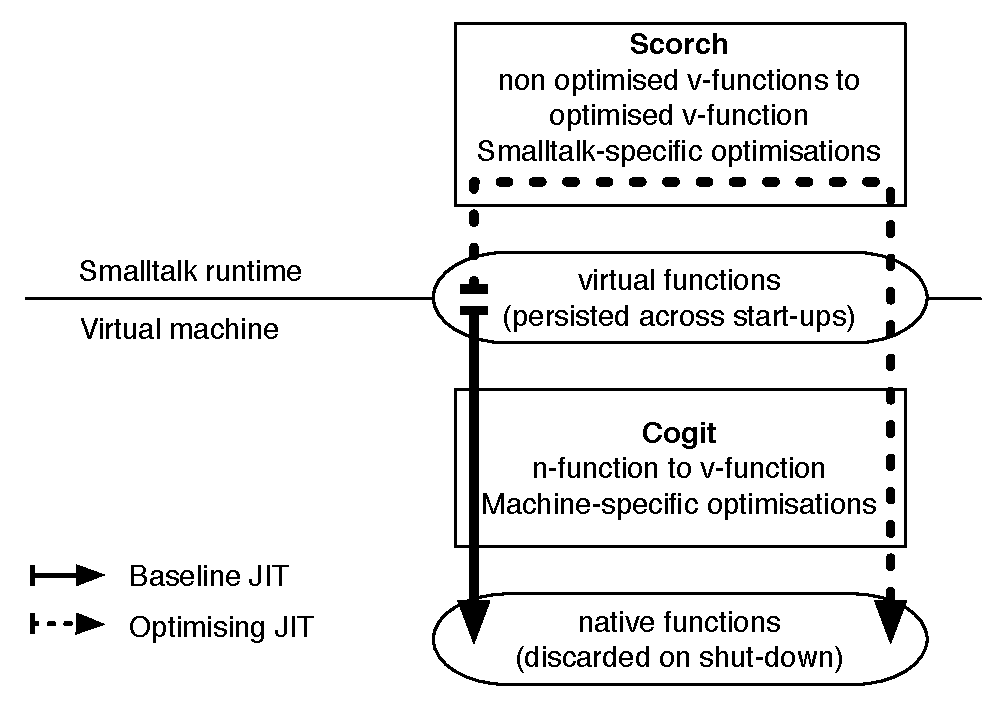
\includegraphics[width=0.8\linewidth]{OptArchitecture}
        \caption{Scorch critical and background modes}
        \label{fig:OptArchitecture}
    \end{center}
\end{figure}

MAYBE MOVE FORWARD ?

%opt intro
Cogit was extended to detect hot spot through profiling counters in non optimised n-functions. When a hot spot is detected, Cogit immediately calls Scorch in Pharo. Scorch then looks for the best v-function to optimise based on the current stack, optimises it and installs the optimised version. To perform optimisation, Scorch may ask Cogit to introspect specific n-functions to extract type information and basic block usage from previous runs. Once installed, the VM can execute the optimised v-function at the next call to the function. As the VM runtime is hybrid between the interpreter and Cogit, the optimised v-function may conceptually be interpreted or compiled by Cogit and then executed as an optimised n-function. In practice, new heuristics were introduced for optimised v-functions to execute them as optimised n-functions from the first run. The details of the function optimisation logic is written in section \ref{sec:functionOptimisation}.

%deopt intro
Due to speculative optimisations, optimised v-functions may contain guards to ensure optimisation-time assumptions are valid at runtime (REF URS HOZLE THING). If a guard fails, the execution stack needs to be deoptimised to resume execution with non optimised code. When an optimised n-frame needs to be deoptimised, Cogit maps the optimised n-frame to a single optimised v-frame. Cogit then provides the optimised v-frame to Scorch, which maps the optimised v-frame to multiple non optimised v-frames. Scorch may discard the optimised v-function if guards are failing too often in it. The execution can then resume using non optimised v-functions. The deoptimisation logic briefly described here is explained in detail in section \ref{sec:functionDeoptimisation}.

TODO maybe ref to related work.

%%%%%%%%%%%%%%%%%%%%%%%%%%%%%%%%%%%%%%%%%%%%%%%%%%%%%%%%%%%%%%%%%%%%%%%%%%%%%%%%%%%%%%%%%%%%%%%%%%%%%%%%%%%%%%%%%%%%%%%%

\section{Overview}

Take exisintg design from intro and move it here.

The existing runtime environment of Pharo relies 

explain existing runtime.

we have interpreter running v-func

we have COgit as bJIT translating v-f to n-f. Cogit use inline cache for perf.

Possible to install code.


Explain new runtime. 

need detect frequently used code in n-func. Extend cogit to do so.

Because Scorch in lang need way to call from hot spot the opt.

Scorch needs to search the stack and pick a func to optimise.

Scorch optimise func with inlining and stuff. To do so it needs runtime info. need extend Cogit to extract data from n-functions.

To support running opt n-func

support new instructions

support for trap call back and deoptimisation 

support for dependency management and discarding



%%%%%%%%%%%%%%%%%%%%%%%%%%%%%%%%%%%%%%%%%%%%%%%%%%%%%%%%%%%%%%%%%%%%%%%%%%%%%%%%%%%%%%%%%%%%%%%%%%%%%%%%%%%%%%%%%%%%%%%%

\section{Function optimisation}
\label{sec:functionOptimisation}

%Intro
Cogit was extended to detect hot spots based on profiling counters. When a hot spot is detected, Cogit triggers a call-back to request Scorch to optimise a v-function based on the current stack. As Pharo is currently single-threaded, the application green thread has to be interrupted to optimise a function. The overall design is then the following: after interrupting the application, Scorch finds a v-function to optimise based on the current stack, optimises it, installs the optimised version, and resumes the application. The optimised v-function installed will be executed at the next call of the function.

\subsection{Optimiser critical and background modes}

%TimeBeforePostPoning: problem so it's required
Scorch's optimiser may however require a significant amount of time to optimise a v-function. Optimising a v-function can take a long time in slow machines or when a pathological function~\footnote{Many compiler algorithms have a good average complexity based on heurisitics but poor worst complexity. A pathological function is a function not matching any heuristic leading to long optimisation time.} is optimised. This can lead to an interruption of the application for an amount time long enough to be noticed by the user. To experiment with the Sista architecture, we worked with the development environment of Pharo (which is written in Pharo). In the case of a user-interface application like this one, it is \emph{very} annoying to see the application interrupted during half a second or more when multiple v-functions long to optimise are optimised in a row. The user interface feels slow, lagging and unresponsive even though the overall code takes less time to execute.

%First solution: timeBeforePostponing, with constraint for long methods
To avoid the problem, we limited the optimisation time to a fixed small time period, configured from the language. For user interface application, we limit it to 40 ms. The limitation is enforced by a high-priority green thread, set to stop the optimiser after the given time period. As the current user interface is refreshing at 50Hz, the optimiser, in the worst case, force the system not to refresh the screen twice. In practice, most v-functions are optimised in less than 40ms. However, some v-functions are still too long to optimise, so an alternative solution is required to optimise them.
%Didn't use frame before not to confuse graphic frames with stack frames.

%idle and postpone
Upon profiling the development tools, as one would expect, we noticed that the application spends a significant amount of time in idle\footnote{An application in idle means it has nothing to do, it is typically waiting for an event to do anything.}. We show for example in figure \ref{fig:ApplicationIdle} that the application is successfully executing code, then idle, then executing code again, etc. In this case, each time an event happen (key stroke, mouse click, etc.), some code is executed, but when no event happens, for example when the developer is reading code, the application is in idle.

\begin{figure}[h!]
    \begin{center}
        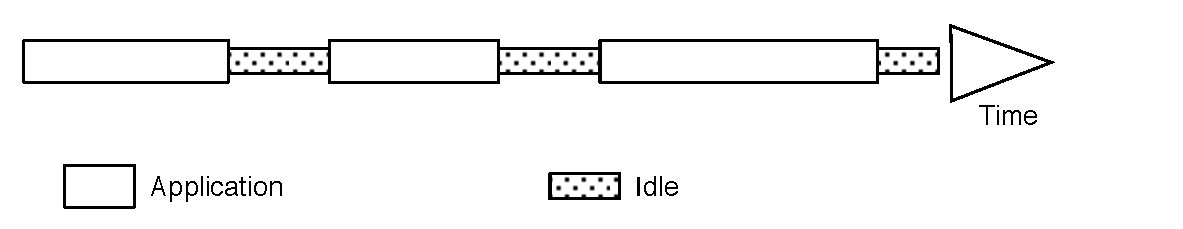
\includegraphics[width=0.95\linewidth]{ApplicationIdle}
        \caption{User interface application idle times}
        \label{fig:ApplicationIdle}
    \end{center}
\end{figure}

%background thread
Based on the profiling result, we introduced a background green thread responsible for optimising the functions too long to optimise in the limited time period allowed. This way, when the application would normally become idle, it starts by optimising such functions and becomes idle when no functions to optimise are remaining. As the background green thread is running at low priority, if the application restarts while an optimisation is being performed, the application green thread preempts the optimisation green thread and no pauses are seen by the user.

%Critical vs background
The optimiser can therefore be run in two mode. When a hot spot is detected, the optimiser is started in \emph{critical mode}. It has a limited time period to optimise a function based on the current stack. If the optimisation takes too long, the function to optimise is added to the background compilation queue. When the application becomes idle, if the background compilation queue is not empty, the optimiser is started in \emph{background mode}. In background mode, the optimiser is run in a low-priority green thread and is preempted by any application green thread. When the optimiser has optimised all the functions in the compilation queue, it stops and the application becomes idle. Scorch's optimiser critical and background modes are represented on figure \ref{fig:ScorchModes}.

\begin{figure}[h!]
    \begin{center}
        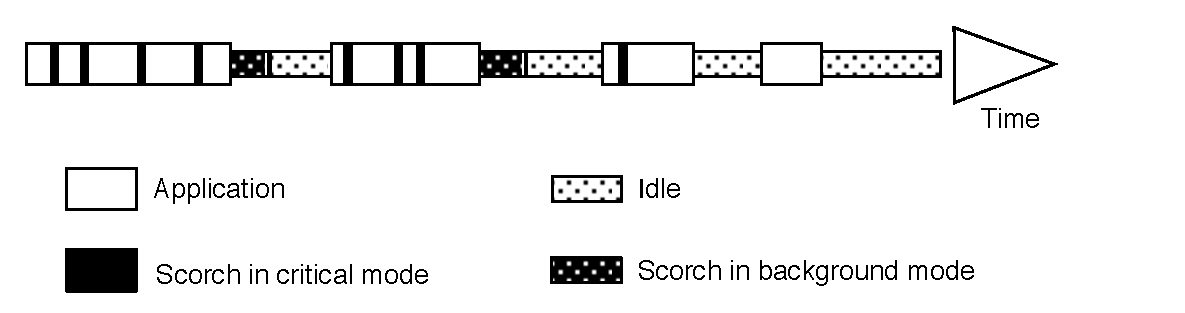
\includegraphics[width=0.95\linewidth]{ScorchModes}
        \caption{Scorch critical and background modes}
        \label{fig:ScorchModes}
    \end{center}
\end{figure}

%Merged with previous paragraph.  Fig explanation, critical vs background mode
%As shown on figure \ref{fig:ScorchModes}, when the application is running, it can be interrupted for a small time window at worst. When the application normally becomes idle, the background green thread starts optimising the functions long to optimise. When no more functions are queued for optimisations, the application becomes idle. In any case, after a while, all critical portions of code have been optimised and the application is usually not interrupted any more while the background green thread has usually no more v-functions to optimise.

\paragraph{Conclusion.}The Scorch optimiser can be run in two modes. In critical mode, it interrupts the application green thread and has a limited time period to optimise a function. If the time limit is not enough, the function's optimisation is postponed to the background mode. In background mode, Scorch optimises code only when the application is idle but has no time limit. This design allow all the application's code to be optimised in a single-threaded environment without the system loosing too much responsiveness.

\subsection{Hot spot management}

%generic profiling counters
Cogit was extended to be able to generate n-functions with profiling counters. Profiling counters allow to detect hot spots and provide information about basic block usage at the cost of a small overhead, detailled in the validation chapter of the thesis. Because of the overhead, Cogit was extended to support conditionnal compilation. Based on a specific bit in the v-function's header, Cogit compiles the v-function with or without profiling counters. Typically, non optimised v-functions, produced by the source code to v-function bytecode compiler~\cite{Bera13a}, are by default compiled to n-functions with profiling counters, while optimised v-functions are compiled without profiling counters. Profiling counters are generated so that the counter is increased by one when the execution flow reaches it and a specific hot spot detection routine is called when the counter reaches a threshold.

%SHOW v-function header format ?

%Counters on branch
Based on \cite{Arn02}, we added counters by extending the way the baseline JIT generates conditional jumps. Counters are added just before and just after the branch. In several other VMs, the counters are added at the beginning of each function. The technique we used allowed us to reduce the counter overhead as branches are 6 times less frequent that virtual calls in Smalltalk. In addition, the counters provide information about basic block usage. Every finite loop requires a branch to stop the loop iteration and most recursive code requires a branch to stop the recursion, so the main cases where hot spots are present are detected.

%hot spot detection - call-back
When a hot spot is detected, a specific Slang routine is called. The routine makes sure the n-frame where the hot spot is detected is reified so it can be introspected from Smalltalk. Then, the routine performs a virtual call with a selector registered from Smalltalk, the reified stack frame as the receiver and the boolean the conditionnal jump was branching on as a parameter. The method activated by the call-back, in Smalltalk, calls the Scorch optimiser.

During optimisation, the bottom frames of the execution stack are used by the Scorch optimiser. The frame above is the call-back frame, followed by the application frame holding the n-function with the hot spot, as shown on figure \ref{fig:HotSpotCallBackStack}.

\begin{figure}[h!]
    \begin{center}
        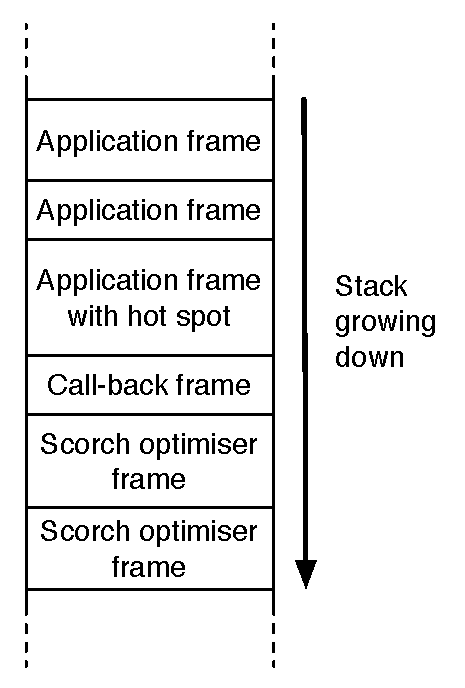
\includegraphics[width=0.35\linewidth]{HotSpotCallBackStack}
        \caption{Stack state during critical mode optimisation}
        \label{fig:HotSpotCallBackStack}
    \end{center}
\end{figure}

%Flag: FRAMEREIFICATION.

%returning from call-back
The profiling counter machine code is generated so that upon return to the n-frame with the profiling counter, the conditionnal branch is performed again on the value returned. This way, if the Smalltalk code resets the profiling counters and returns the boolean passed by argument to the call-back, the application execution is resumed by performing one more time the branch with the same boolean.

%WARNING ! What happen when conditionalBranchTrip and reification.

\subsection{Scorch optimiser}

The Scorch optimiser is activated by the call-back and has access to the reified stack. Scorch firstly analyse the stack and finds the best function to optimise. Then, it generates, either directly in critical mode or indirectly through background mode an optimised v-function and installs it for further uses.

%TO REMOVE
%We call the \emph{tripping function} the function where the hot spot is detected, because a counter has "tripped" in this function.

\paragraph{Stack search.}
\label{ss:stackSearch}

%Function selection, bottom is bad
When a hot spot is detected, Scorch is activated and has access to the reified stack. A naive approach would be to always optimise the function where the hot spot is detected and not to search the stack at all. Unfortunately, this heuristic would be terrible for Smalltalk. An important part of the execution time is due to the extensive use of closures. More specifically, most loops in the executed code, assuming the code respects standard Smalltalk coding conventions, are using closures. To efficiently remove the closure overhead, the closure needs to be inlined up to its enclosing environment to remove both the closure creation and the closure activation. If the function where the hot spot is detected is either activating closures or a closure activation itself, then optimising it won't gain that much performance because the closure creation and activation execution time will remain.

%Function selection, bottom or home is bad
Another approach, a bit less naive, would be to optimise the function where the hot spot is detected if it is a method, and the enclosing environment's function if it is a closure, in an attempt to remove closure overhead. Yet, this heuristic still does not solve the most common case of the problem. To illustrate the problem, let's look at a simple example with a loop over an array.

%array loop example. descr exampleArrayLoop
In the code sample in figure \ref{fig:ExampleCode}, \ct{exampleArrayLoop} is a method installed in the class \ct{ApplicationClass}. Its method body consists of a loop over an array, the array being an instance variable. To loop over an array, Smalltalk provides high level construct such as \ct{do:}. In this case, \ct{do:} is very similar to \ct{foreach} in other languages and allows to iterate over the array while providing at each iteration of the loop the array's element in the variable \ct{element}. The \ct{do:} method, installed in \ct{Array}, takes a single argument, a closure, which is evaluated using \ct{value:} at each iteration of the loop. The parameter of the closure activation is \ct{self at: i}, which represent the access to the element \ct{i} of the array. During the closure evaluation, the bottom three frames are the closure activation, the frame for \ct{Array >> do:} and the frame for \ct{ApplicationClass >> exampleArrayLoop} as shown on figure \ref{fig:ExampleLoopStack}.

\begin{figure}[h!]
    \begin{center}
        \begin{code}
        	ApplicationClass >> exampleArrayLoop
        	    array do: [ :element | FileStream stdout nextPutAll: element printString ].
        		
        	Array >> do: aClosure
        	    1 to: self size do: [:index | aClosure value: (self at: index)].
        \end{code}   
	\caption{Example code}
        \label{fig:ExampleCode}
    \end{center}
\end{figure}

\begin{figure}[h!]
    \begin{center}
        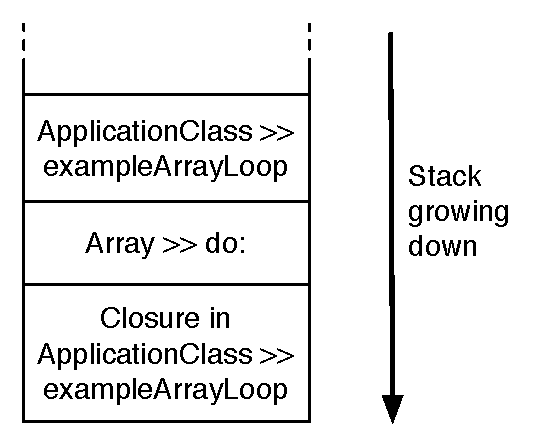
\includegraphics[width=0.42\linewidth]{ExampleLoopStack}
        \caption{Example stack during closure execution}
        \label{fig:ExampleLoopStack}
    \end{center}
\end{figure}

%descr do:
The method \ct{Array >> do:} is using a special selector, \ct{to:do:}, which is compiled by the bytecode compiler to a loop, in a similar way to \ct{for} constructs in other programming languages. In fact, the \ct{Array >> do:} method body is a loop from 1 to the size of the array, evaluating the closure at each iteration for each element in the array. At each iteration, the current value of index is tested against the size of the array, and when that value is reached the loop is exited.

%profiling counter location
As discussed in the previous section, profiling counters detect frequent portion of code on branches. Each finite loop has a branch to either keep iterating over the loop or exit the loop. In the example, it means that the method \ct{Array >> do:} has a profiling counter on the branch testing the value of the index against the size of the array. The rest of the code, in the two methods and in the closure, have no other profiling counters.

%closure issue and why to pick next function
The hot spot is going to be detected on the profiling counter, hence in the method \ct{Array>>do:}. If Scorch optimised the \ct{Array>>do:} method, it cannot know what closure will be executed as the closure is an argument, while an important part of the execution time is spent creating and evaluating the closure. However, if \ct{Array>>do:} gets inlined into \ct{ApplicationClass>>exampleArrayLoop}, the closure evaluated would be known to be the closure \ct{[ :element | FileStream stdout nextPutAll: element printString ]}. Hence, to gain maximum performance, the optimiser should decide to optimise \ct{ApplicationClass>>exampleArrayLoop} and inline both the \ct{Array>>do:} method and the closure evaluation (\ct{value:}). 

%detail of the problem
In this case, the hot spot is detected in \ct{Array>>do:}. The hot spot is therefore detected in a method, not a closure. Naive heuritics would have chosen to optimise \ct{Array>>do:}, while it is better to select the caller stack frame's function.

%closure last explanation
Overall, because of the extensive use of closures, the optimiser almost never chose to optimiser the function where the hot spot is detected. It usually walks up a few frames to find the best function to optimise. 

\paragraph{Optimised v-function generation.}
Once Scorch has selected the v-function to optimise, it generates an optimised v-function. It attempts to do it immediately, within a limited amount of time. If it fails to do it, it postpones the optimisation to background mode. The function's optimisation and installation is using the same code in both cases, so we will discuss only the critical mode optimisation in the following paragraphs.

Scorch's optimiser is implemented with traditional compiler optimisation techniques. It decompiles the v-function to optimise into a single static assignment intermediate representation, represented in the form of a control flow graph. Specific instructions that may require deoptimisation of the optimised frame have deoptimisation metadata attached which is updated during the optimisation passes to still refer to the correct values. During decompilation, Scorch asks Cogit to introspect the n-function corresponding to the v-function decompiled. If such a n-function exists, Cogit provides type information for each virtual call based on the data present in each inline cache and provide basic block usage based on the profiling counter values. The intermediate representation is annotated with this runtime information.

%The same intermediate representation is used during the whole optimisation process.

Scorch's optimiser performs Smalltalk specific optimisations, very similar to the object-oriented specific optimisations present in other optimising JITs. Guided by the information provided by Cogit, Scorch speculates on receiver types for each virtual call to determine what v-function to inline. Each inlined v-function is decompiled to the same intermediate representation, annotated with runtime information the same way and merged into the same control flow graph. Each inlined function requires the insertion of a deoptimisation guard, to stop using the optimised code at runtime if the receiver type assumptions are not valid anymore. Once the inlining phasis is finished, Scorch's optimiser performs standard optimisations such as array-bounds check elimination with the ABCD algorithm~\cite{Bodi00a}, global value numbering, loop invariant code motion and postpone allocation of objects not escaping the optimised v-function from runtime to deoptimisation time (or completely removes the allocation if the object is never required for deoptimisation).

The back-end is the only non conventional part of the optimiser. Scorch needs to generate an optimised v-function and not an optimised n-function. Most intermediate representation instructions map one to one to the extended bytecode set instructions. However, as the bytecode set is stack-based, the back-end needs to map each used intermediate representation instruction value either to a value on stack or a temporary variable. The deoptimisation metadata needs to be updated accordingly.

Lastly, the back-end generates an optimised v-function. For each point where deoptimisation could be requested (typically, failing guards, but also each virtual call for debugger support), the optimised v-function has metadata attached to reconstruct the stack with non optimised v-functions.

\paragraph{Installation.}
If the optimisation has been done in time in critical mode or has simply been done in background mode, the optimised v-function can be installed. It is installed in the method dictionary of a class if this is a method, or in a method if it's a closure. If an optimised method is installed, the installation explicitely requests the VM to flush the caches dependent of this installation so it can be used at next call (the global look-up cache for the interpreter and the inline caches).

In addition, the dependencies are installed in the dependency manager so that if new code is loaded, code that may be dependent is discarded.

Once installed, conceptually, the VM runs the optimised v-function as a normal v-function. The first few runs can be interpreted and the subsequent runs use the n-function produced by Cogit. The only difference is that optimised v-functions have access to additional operations, but those operations are supported both by the interpreter and by Cogit. The first version we had running was working exactly this way.

We then added a cheap heuristic to encourage the execution of optimised v-functions as n-functions. Optimised v-functions have a bit set in their header to tell Cogit not to compile profiling counters when generating their corresponding n-function. If this bit is set, we added the heuristic that the interpreter asks Cogit to compile it at the first run and immediately uses the n-function instead of doing so after a couple of interpretations.

In any case, the VM still needs to support the interpretation of optimised v-functions. Indeed, in very rare cases, Cogit cannot temporarily generate a n-function for the given v-function. For example, as the native code zone for n-functions has a fixed size of a few megabytes, it can happen that Cogit tries to compile a v-function while relinking a polymorphic inline cache~\cite{Holz91a} of another n-function. If there is not enough room in the machine code zone, a compaction of the machine code zone has to happen while relinking. It is not easy to compact the machine code zone at this point as it can happen that the polymorphic inline cache or the n-function holding it is discarded. To keep things simple, in this situation, we postpone the machine code zone compaction to the next interrupt point and interpret the v-function once. The interpretation of optimised v-functions, even if uncommon, is required for the VM to execute code correctly.  

%%%%%%%%%%%%%%%%%%%%%%%%%%%%%%%%%%%%%%%%%%%%%%%%%%%%%%%%%%%%%%%%%%%%%%%%%%%%%%%%%%%%%%%%%%%%%%%%%%%%%%%%%%%%%%%%%%%%%%%%

\section {Function deoptimisation}
\label{sec:functionDeoptimisation}

%intro
The deoptimisation of the execution stack is similar to other VMs \cite{Fin03a, Holz92a}. The optimised frame is on stack and is in most case a n-frame~\footnote{In very uncommon cases, the VM may decide to interpret an optimised v-function, leading to the presence of an optimised v-frame.}. The optimised frame cannot be used any more because an optimisation time assumption is invalid at runtime (a deoptimisation guard has failed) or the optimised function was discarded (by the debugger or because of new code loading). Deoptimising the stack requires the mapping of the optimised frame to multiple non optimised v-frames. 

%Main difference
In our architecture, deoptimisation is done in two steps as shown on figure \ref{fig:SFDeoptimisation}. Firstly, Cogit deoptimises the optimised n-frame to a single optimised v-frame. This step is not performed in the uncommon case where deoptimisation happens already from an optimised v-frame. For the rest of the section, we assume that the optimised frame is a n-frame, the other case being uncommon and being implemented simply by ignoring this first step. Secondly, Scorch deoptimises the optimised v-frames to multiple non optimised v-frames.

\begin{figure}[h!]
    \begin{center}
        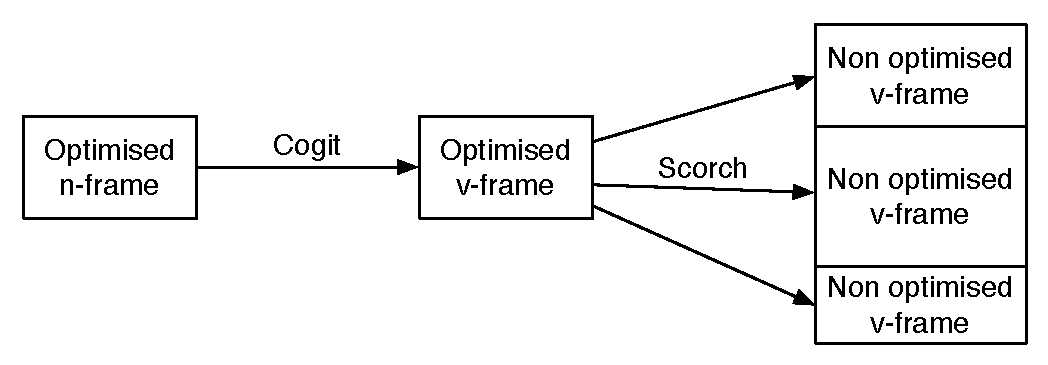
\includegraphics[width=0.8\linewidth]{SFDeoptimisation}
        \caption{Stack frame deoptimisation in two steps}
        \label{fig:SFDeoptimisation}
    \end{center}
\end{figure}

%only stack deopt
When discussing deoptimisation, we deal only with stack recovery (deoptimisation of the optimised frame to the non optimised v-frames). The non optimised v-function is always present and never discarded, so it can be directly set in the non optimised v-frames restored. There is no such thing in our design and implementation as reconstructing non optimised v-function from optimised v-function based on deoptimisation metadata. As far as we know, modern VMs such as V8~\cite{V8} always keep a non-optimised version of each function, so we believe the memory footprint impact of keeping them is acceptable.

\subsection{Deoptimisation management}

%Intro + 2 cases.
Deoptimisation can happen in two main cases. On the one hand, Scorch's optimiser inserts guards(CITE URS OU Dubois) to ensure assumption speculated at optimisation time are valid at runtime, such as the speculation on types. Such guards can fail, requiring deoptimisation of the execution stack to keep executing the application correctly. On the other hand, Smalltalk code can request deoptimisation of the code when manipulating the stack (typically the debugger's code does it).

\paragraph{Guard failure.} When a guard fails, the native code generated by Cogit calls a specific routine in Slang to perform the deoptimisation of the stack. The routine makes sure the frame with the tripping counter is reified so it can be introspected from Smalltalk. Then, the routine performs a virtual call with a selector registered from Smalltalk and the reified stack frame as the receiver. The Smalltalk code lastly calls Scorch deoptimiser's to restore the non optimised stack.

During deoptimisation, the bottom frames are used by the deoptimiser. Just above is a frame for the activation of the virtual call performed by the routine followed by the optimised frame requesting deoptimisation, as shown on figure \ref{fig:DeoptCallBackStack}.

\begin{figure}[h!]
    \begin{center}
        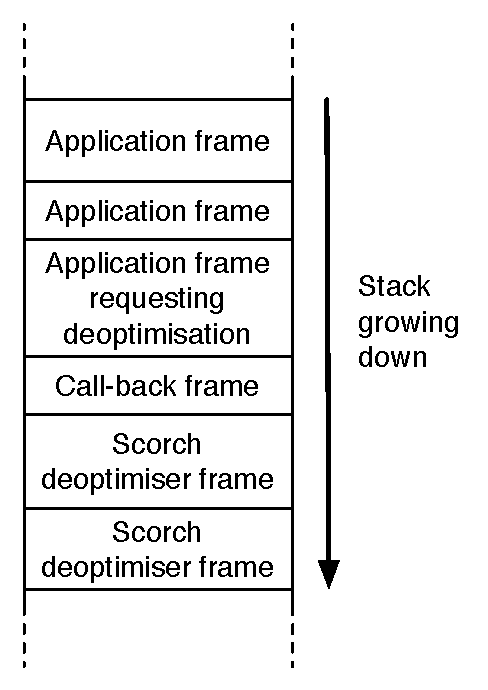
\includegraphics[width=0.4\linewidth]{DeoptCallBackStack}
        \caption{Stack state during guard deoptimisation}
        \label{fig:DeoptCallBackStack}
    \end{center}
\end{figure}

%low-level stack banging issue, in Slang ?
%Flag: FRAMEREIFICATION.

\paragraph{Smalltalk code deoptimisation.}The Smalltalk code can request deoptimisation of specific frames to perform specific operations such as debugging. In this case, the situation is different because:
\begin{enumerate}
	\item The frame to deoptimise is in the middle of the application frames. Instead of having the call-back and deoptimiser frames below the frame to deoptimise on stack, other application frames are present.
	\item The instruction pointer is not on a guard instruction. Although, all instructions where deoptimisation can happen are annotated with deoptimisation metadata, so having the instruction pointer on a non guard instruction does not really change much.
\end{enumerate}

\subsection{Scorch deoptimiser}

%deopt through metadata 
Cogit has reified the optimised n-frame to an optimised v-frame, hence, Scorch's deoptimiser access the optimised v-frame. The frame is necessarily activated on a virtual instruction which is annotated with deoptimisation metadata. The metadata consists of a list of objects to materialize, which allocation have been postponed from runtime to deoptimisation time. As v-frames and closures are reified as objects in Smalltalk, part of those objects to rematerialize are non optimised v-frames and closures. For each field of each object, the metadata specifies if the value is a specific constant, a value to fetch in the optimised v-frame or a reference to one of the other rematerialized object.

\paragraph{Stack edition.}

Once all the non optimised v-frames are reconstructed, the execution stack needs to be edited to use them. This is done using the stack manipulation APIs. Basically, the VM split the current stack page in two, copying one part on another stack page. Deoptimised frames are present in the middle in their single context form, in a similar way to frame divorces described in the previous chapter and as shown in figure \ref{fig:DeoptStacks}.

\begin{figure}[h!]
    \begin{center}
		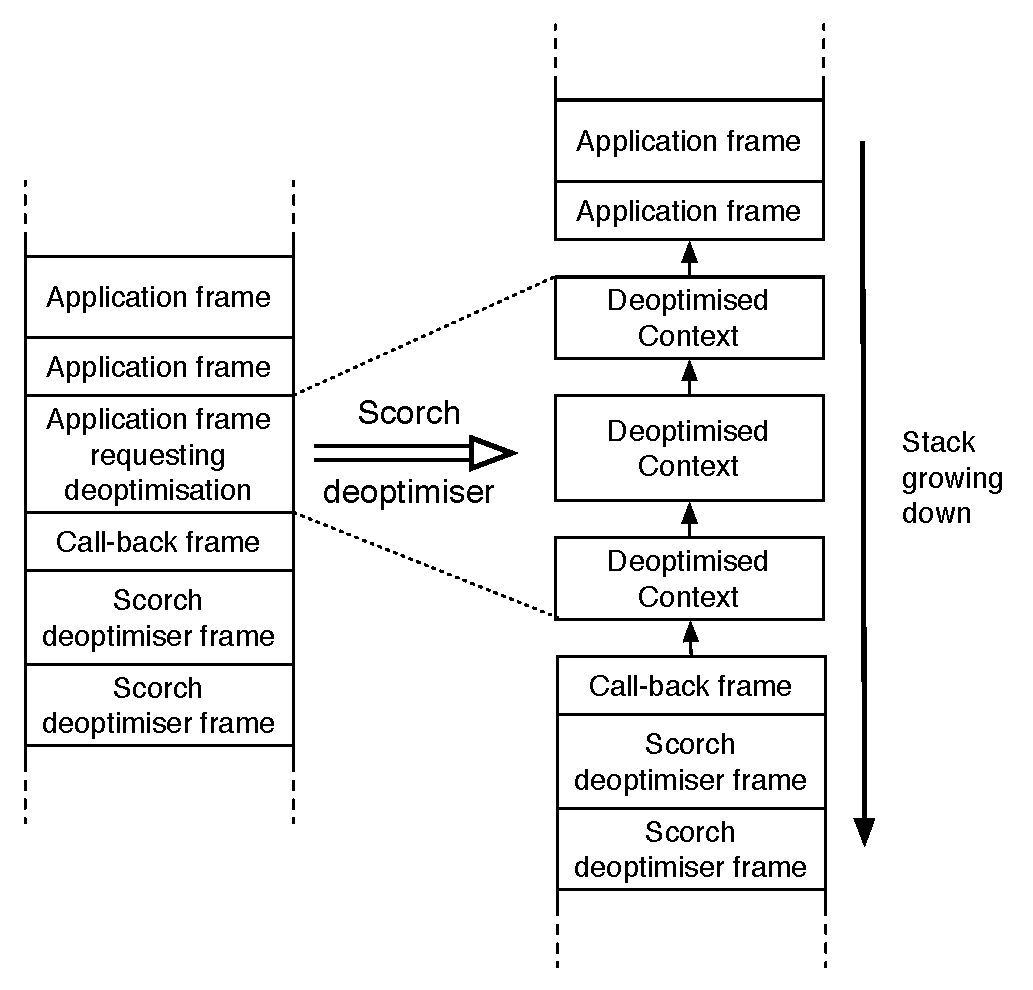
\includegraphics[width=0.80\linewidth]{DeoptStacks}
        \caption{Stack edition}
        \label{fig:DeoptStacks}
    \end{center}
\end{figure}

\paragraph{Discard functions.} When new non optimised functions are installed (for example when a library is loaded), optimisation assumptions may be invalidated because some look-up results cannot be guaranteed any more. In this case, we cannot really iterate over the whole stack and deoptimise all the frames holding invalidated code as it would take a long time (especially multiple stack manipulations may take a while). Instead, Scorch mutates the discarded optimised v-function to hold only guard failures virtual instructions, so optimised v-frames would always trigger deoptimisation upon return. In addition, Scorch requests Cogit to patch all return native instruction pointers of all optimised n-frames representing discarded function activations to a pointer to a specific routine which will trigger deoptimisation upon return.

\paragraph{Execution restart.}

If the deoptimisation happened due to a guard failure (or due to a return to a discarded function), the application needs to resume execution once deoptimisation is performed. In this case, the application frame is just above the call-back frame so returning should resume execution. There is one little detail, a return instruction in Smalltalk pushes the returned value on the caller stack. The deoptimisation call-back returns the top value of the bottom deoptimised frame to resume execution. The bottom deoptimised frame is guaranteed not to be empty as deoptimisation can be only in position in the code where there is necessarily something on stack.

%In those cases, the first deoptimiser frame is just below the bottom restored non optimised v-frame. Returning from the deoptimiser frame to the application is not as easy as for the optimiser call-back. The optimiser is always triggered on a conditional branch and conditionnal branches require a value to test to be on stack. Hence, the optimiser could simply return the value to test and the execution resumes just before the branch. 

%In the case of deoptimisation, the application stack frame could be restored on many different instructions. Especially, it could be restored at an instruction where no value is on stack. Hence to return to the application, the deoptimiser has to perform a special return instruction, which resumes the caller frame execution without pushing any value on its frame.

%%%%%%%%%%%%%%%%%%%%%%%%%%%%%%%%%%%%%%%%%%%%%%%%%%%%%%%%%%%%%%%%%%%%%%%%%%%%%%%%%%%%%%%%%%%%%%%%%%%%%%%%%%%%%%%%%%%%%%%%

\section{Related work}

Take prev section arch in order and explain why we pick one design other another and what are different

function based JIT and not meta tracing JIT - on top of existing, pb with stack search.

sharing back-ends - we believe we can waste only limited performance by reusing Cogit while decreasing maintenance cost

native threads - we are single threaded so that's how we do it.

%%%%%%%%%%%%%%%%%%%%%%%%%%%%%%%%%%%%%%%%%%%%%%%%%%%%%%%%%%%%%%%%%%%%%%%%%%%%%%%%%%%%%%%%%%%%%%%%%%%%%%%%%%%%%%%%%%%%%%%%

\paragraph{Conclusion.}
% \section {Conclusion} ?


\ifx\wholebook\relax\else
    \end{document}
\fi